\chapter{Detection}
\label{chap:Detection}

\section{Analysis}

\section{Supervised Learning}

\subsection{Random Forests}

\subsection{Decision Trees}
However, to split the data for the anomalies, we need to decide which input parameter will be used to make the first split, the root node. The Gini index measures the probability of a data sample being wrongly classified at a given node. This can be calculated with Eq~\ref{eq:Gini index}.

\begin{equation}
	GI = 1 - \sum_{i = 1}^{n}{(P_i)^2}
	\label{eq:Gini index}
\end{equation}

The operator split that produces the lowest Gini index provides the purest split and will be used as the root node. For our use case, the CART algorithm will be used to optimise the decision tree, which also considers the most prominent information gain to construct the decision tree. Figure~\ref{fig:DecisionTree} is a graphical representation of the decision tree developed to classify anomalies. The depth of a decision tree determines how many splits occur from the root node to the leaf node the furthest from the first split. If the depth is unspecified, the decision tree will split until all the data samples are perfectly split into anomalous and normal data samples. However, the larger the depth, the more biased the decision tree is to the training data. This depth can be altered to optimise the efficiency and accuracy of the decision tree.
\begin{figure}[!hbt]
	\centering
	\import{Figures/}{DecisionTree.pgf}
	\caption{Decision Tree}
	\label{fig:DecisionTree}
\end{figure}

\subsection{Support Vector Machines}

\section{Unsupervised Learning}

\subsection{Isolation Forests}
This unsupervised learning method is based on the principle of isolating data points by slicing the data with random conditions \cite{TonyLiu2008}. The data is randomly split into specified sample sizes with a randomly selected dimension and a randomly selected cut-off value. For each sample size the data must be split until each data point within the sample is isolated from all other data points. Training of a single tree is completed when all the data points are isolated and this training must be repeated for all the data samples, however many are predefined. 

The distance measured from the first split the \emph{tree top} to the isolated data point is used to determine whether a data point is anomalous or not \cite{Hariri2021}. The logical reasoning for support of this algorithm is that data points which are non-anomalous will be more closely related and hence have more splits to separate the data points until isolation is achieved. Therefore, the distance from the tree top for non-anomalous data points will be longer than anomalous data points which will have a shorter distance from the tree top. Therefore non-anomalous data points are closer to the \emph{root}. 

Figure~\ref{Figure-Isolation_Forest} demonstrates the splitting of the data points until isolated. Each split or \emph{branch} only splits the data into two groups. After training multiple trees, a single data point is "sent through the forest" and the distance from the tree top for each tree is calculated and the average of all the trees are used to calculated the average distance for the data point. Using a threshold for the distance, the data point is classified as anomalous or not.


\begin{figure}[!hbt]
	\centering
	\import{Figures/}{IsolationForest.pgf}
	\caption{Isolation Forest}
	\label{fig:IsolationForest}
\end{figure}
\begin{figure}[h!tb]
	\centering
	
	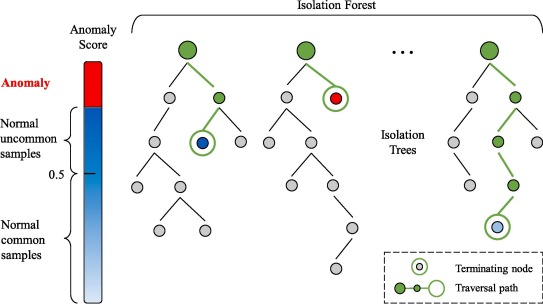
\includegraphics[width=10cm]{fig/Isolation_Forests} % not necessary to give extension - now you can shift between compiling to ps or to pdf without any problems
	
	\caption[Isolation Forest]{Isolation Forests \cite{Chen2020}}
	\label{Figure-Isolation_Forest} 
\end{figure}

The anomaly score is calculated with Eq~\ref{Eq-Isolation_anomaly}
\begin{equation}
	s(x,n) = 2^{-E(h(x))/c(n)}
	\label{Eq-Isolation_anomaly}
\end{equation}
where $E(h(x))$ is the average value of the distance measured from the tree top for a single data point in all the trees \cite{Hariri2021} and $n$ is the size of a data sample used to train a single tree. For the distance to be normalized, $c(n)$ --- the mean distance from the tree top in an unsuccessful search in a \emph{Binary Search Tree} (BST) --- is used and is calculated as 
\begin{equation}
	c(n) = 2H(n-1) - \frac{2(n-1)}{n}.
	\label{Eq-normalizing_isolation}
\end{equation}
$H(i)$ in Eq~\ref{Eq-normalizing_isolation} is the harmonic number and is estimated with Euler's constant as 
\begin{equation}
	H(i) \approx ln(i) + 0.5772156649.
	\label{Eq-H_i}
\end{equation}
Isolation Forests, however have multiple issues, since it splits data in rectangles as seen in Figure~\subref{Figure-ExtendedvsNormal_first}. This is due to the slicing algorithm selecting a feature, $x$ and a cut-off value, $v$. Consequently, the data is either split vertically or horizontally --- if seen as a two dimensional dataset. This split method is unable to categorise complex data structures. These issues however are addressed by \cite{Hariri2021} and led to the \emph{Extended Isolation Forest} algorithm.

The extended isolation forest algorithm generalises the isolation forest algorithm by applying a slope to each slice. Data points are therefore divided into two groups depending on the "side" of the plane or slice as seen in Figure~\subref{Figure-ExtendedvsNormal_second}.

\begin{figure}[h!tb]
	\centering
	
	\subfloat[][Isolation Forest Slicing example]{
		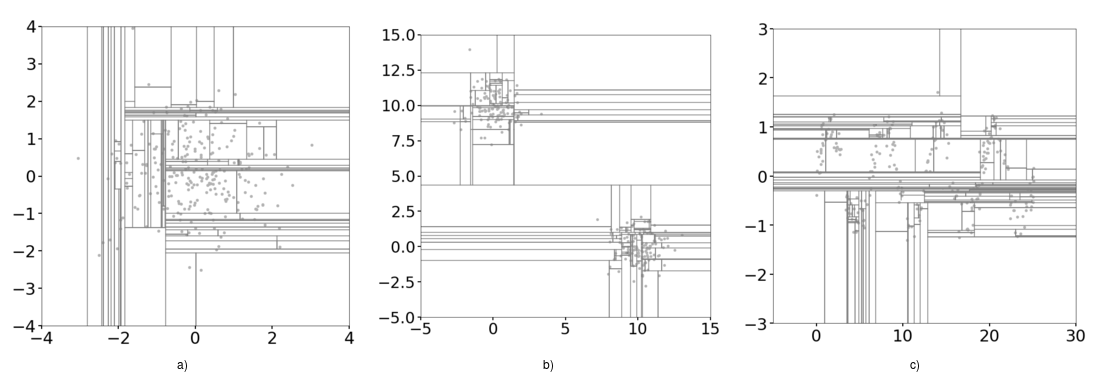
\includegraphics[trim = 0 0 725 0, clip = true, width=7cm]{fig/Isolation_forest_slicing}
		\label{Figure-ExtendedvsNormal_first}
	}
	\quad
	\subfloat[][Extended Isolation Forest Slicing example]{
		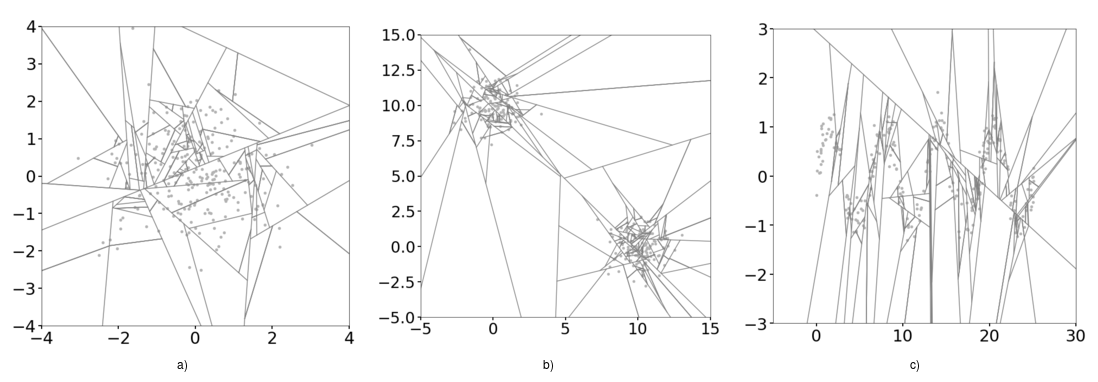
\includegraphics[trim = 0 0 725 0, clip=true,width=7cm]{fig/Extended_Isolation_forest_slicing}
		\label{Figure-ExtendedvsNormal_second}
	}
	\caption[Slicing of Isolation Forest]{The slicing of Isolation Forest vs Extended Isolation Forest}
	\label{Figure-ExtendedvsNormal}
\end{figure}

It is evident that applying an angle of $0\degree$ to all the slices the general algorithm of the extended isolation forest produces the standard isolation forest algorithm where planes or slices are perpendicular to the axis of the randomly selected feature, $x$.

\subsection{Local Outlier Factor}
Most algorithms for anomaly detection are based on a metric which accounts for the entire dataset~\cite{breunig2000lof}. However, many anomalies are identifiable in relation to the local neighbourhood of data points and not the overall dataset. Therefore, \cite{breunig2000lof} developed the local outlier factor \(LOF\) algorithm that provides a measure of a data point's "outlierness". This implies that a data point is not classified as an anomaly or not, but a local outlier factor is calculated to determine how much a data point is distantiated from it's $k$-nearest neighbours. This is clearly demonstrated in Figure~\ref{Figure-LOF_measure} where the data points which are clustered together have smaller LOF's than data points which are removed from the highly dense areas.

\begin{figure}[!hbt]
	\centering
	\import{Figures/}{LOF.pgf}
	\caption{Plane perpendicular to $\mathbf{R}_{SE}$ and at center of earth}
	\label{fig:localOutlierFactor}
\end{figure}

To calculate the LOF, the $k$-distance must be calculated and also the local reachability density \(lrd\). The $k$-distance, is the $k^{th}$ ranked $distance(o,p_i)$. Where $distance(o,p_i)$ is the distance between data point $o$ and any data point $p_i$, with $i \in N$, where $N$ is the number of data points within the dataset with a minimum value of $MinPts$. To reduce fluctuations in the $distance(o,p_i)$ the distance between $o$ and $p_i$ is replaced with 
\begin{equation}
	max \{distance(o,p_i), k\text{-distance}\} 
\end{equation}
and will henceforth be referred to as the reachability distance~\cite{breunig2000lof}. The $lrd$ of a data point, $p$, is calculated as 
\begin{equation}
	lrd_{MinPts}(p) = 1/\left(\frac{\sum\limits_{o \in N_{MinPts}(p)}^{} reach\-dist_{MinPts}(p,o)}{|N_{MinPts}(p)|}\right)
	\label{Eq-lrd}
\end{equation}
and denotes "the inverse of the average reachability distance based on the $MinPts$-nearest neighbours of the $p$" --- \cite{breunig2000lof}. Eq~\ref{Eq-lrd} enables the calculation for the $LOF$ of point $p$ as shown in Eq~\ref{Eq-LOF}
\begin{equation}
	LOF_{MinPts}(p) = \frac{\sum\limits_{o \in N_{MinPts}(p)}^{}\frac{lrd_{MinPts}(o)}{lrd_{MinPts}(p)}}{|N_{MinPts}(p)|}
	\label{Eq-LOF}
\end{equation}
The rule of thumb for detecting an outlier is that when the LOF is larger than 1, then the point is considered an outlier with respect to its neighbourhood. This however is not fixed and the threshold can be changed depending on the application.
This method is aimed at producing a measure of the "outlierness" of a data point within a local neighbourhood and not for all the data points. This method will thus be implemented for the satellite anomaly detection, since it will detect anomalies within the two neighbourhoods produced by the eclipse during orbit. This method will also be able to detect measurements of earth sensors, sun sensors and magnetometers that drastically change from the previous orbital data. For example in Fig~\ref{Figure-Satellite_orbit} it is evident that the LOF will be comparatively larger for the red data points, which are anomalies, to the blue data points that are the normal orbit of the satellite.

\begin{figure}[h!tb]
	\centering
	\begin{tikzpicture}
		\begin{axis}[title = Earth Sensor During Multiple Orbits]
			\addplot3 table [x =Earth x, y = Earth y, z=Earth z, col sep=comma, only marks, scatter, blue, fill opacity=0.1, draw opacity = 0]{Data/3D_orbit.csv};
			\addplot3 table [x =Earth_anomaly x, y = Earth_anomaly y, z=Earth_anomaly z, col sep=comma, only marks, scatter, red, fill opacity=0.1, draw opacity = 0]{Data/3D_orbit.csv};
		\end{axis}
		\label{Figure-Satellite_orbit}
	\end{tikzpicture}
\end{figure}

\section{Summary}
